\documentclass[border=3pt]{standalone}

%Drawing
\usepackage{tikz}

%Notation
\usepackage{physics}
\usepackage{bm}

%Tikz Library
\usetikzlibrary{calc, patterns}

%Newcommand

%%Midline Label
\newcommand{\midlinelabel}[3]{
   \node[shift={(3.5,0)}] (midlabel) at ($ (#1)!.5!(#2) $) {#3};
   \draw[latex-,thick] ($(#1)+(3.5,0)$) --  (midlabel);
   \draw[-latex,thick] (midlabel) -- ($(#2)+(3.5,0)$);
}



\begin{document}
	
	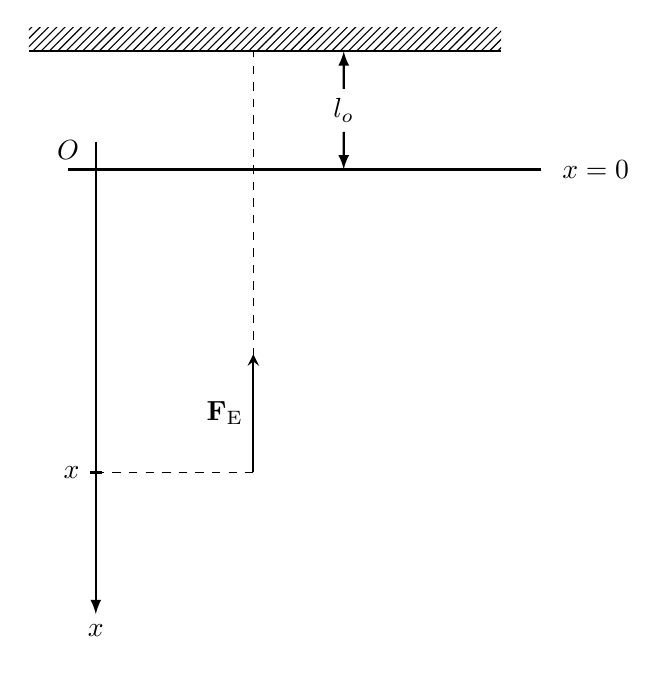
\begin{tikzpicture}
%		%Grid
%		\draw[thin, dotted] (0,0) grid (8,8);
%		\foreach \i in {1,...,8}
%		{
%			\node at (\i,-2ex) {\i};	
%		}
%		\foreach \i in {1,...,8}
%		{
%			\node at (-2ex,\i) {\i};	
%		}
%		\node at (-2ex,-2ex) {0};
		
		%Coordinate
		\coordinate (A) at (0,8);
		\coordinate (A') at ($(A)+(0.5,0)$);
		\coordinate (B) at (0.5,6.5);
		\coordinate (C) at ($(B)+(1em,1em)$);
		\coordinate (D) at ($(C)+(0,-6)$);
		\coordinate (E) at ($(C)!0.7!(D)$);
		\coordinate (F) at ($(E)+(2,0)$);
		\coordinate (G) at ($(B)!0.5!(C)$);
%		%%Nodes
%		\node at (A) {A};
%		\node at (B) {B};
%		\node at (C) {C};
%		\node at (D) {D};
%		\node at (E) {E};
%		\node at (F) {F};
		
		%Lines
		\draw[thick] (A) -- +(6,0);
		\draw[thick] (B) -- +(6,0);
		\draw[-latex, thick] (C) -- (D) node[below] {$x$};
		\draw[thick] (E) -- +(0.5ex,0) -- +(-0.5ex,0) node[left] {$x$};
		%%Dashed
		\draw[dashed] (E) -- (F);
		\draw[dashed] (F) -- +(0,5.34);
		%%Fill
		\fill[pattern=north east lines] (A) rectangle +(6,0.3);
		
		%Vectors
		\draw[-stealth, thick] (F) -- +(0,1.5) node[midway, left] {$\vb{F}_\mathrm{E}$};
		\midlinelabel{B}{A'}{$l_o$}
		
		%Nodes
		\node at ($(B)+(0,0.25)$) {$O$};
		\node at ($(B)+(6.7,0)$) {$x=0$};
	\end{tikzpicture}
	
\end{document}
